\documentclass[11pt]{article}
\usepackage[margin=1in]{geometry}
\usepackage{booktabs}
\usepackage{graphicx}
\usepackage{amsmath}
\usepackage{float}
\usepackage{hyperref}

\title{EE/CS 148B HW2: Profiling and Reasoning}
\author{Dhruv Sheth}
\date{}

\begin{document}
\maketitle

%% -------------------------------------------------------
All profiling and training was run on a RunPod A100-SXM 80GB instance.

\section*{2.3 Benchmarking}

Table~\ref{tab:bench} shows forward and forward+backward times on an A100
(5 warmup steps, 10 measured steps, \texttt{ctx\_len=128}, \texttt{batch=4}).

\begin{table}[h]
\centering
\caption{Latency in milliseconds on A100.}
\label{tab:bench}
\begin{tabular}{lcccc}
\toprule
Model  & Fwd fp32 & Fwd bf16 & Fwd+Bwd fp32 & Fwd+Bwd bf16 \\
\midrule
small  & 13.2     & 14.2     & 30.2         & 33.8 \\
medium & 20.1     & 22.1     & 49.9         & 57.1 \\
large  & 39.5     & 42.1     & 127.2        & 115.4 \\
\bottomrule
\end{tabular}
\end{table}

\begin{figure}[H]
\centering
\includegraphics[width=0.75\textwidth]{benchmark.pdf}
\caption{Forward and forward+backward latency (ms/step) on A100 for all model sizes.}
\end{figure}

The backward pass takes roughly 2--3$\times$ longer than forward, which makes
sense: backprop stores activations for gradient computation.
BF16 is not faster than FP32 for smaller models because at these batch sizes
compute is not the bottleneck.
Without warmup, times are 5--10$\times$ higher due to CUDA kernel compilation
and caching not having happened yet.
One or two warmup steps help, but 10 steps gives stable numbers.

%% -------------------------------------------------------
\section*{2.4 Nsight Profiling}

The dominant CUDA kernel is \texttt{ampere\_sgemm} (matrix multiply), called
$N_\text{layers} \times 6$ times per forward pass: QKV projections, output
projection, and the two FFN linear layers.
Softmax and LayerNorm kernels also appear but together account for less than
10\% of runtime.
During forward+backward, the matmul fraction drops slightly as gradient
reduction kernels become more significant.

%% -------------------------------------------------------
\section*{2.5 Mixed Precision}

FP32 is the default: all parameters and accumulation in full precision.
Under autocast, model parameters are cast to FP16, but LayerNorm stays in FP32
because it is sensitive to precision.
BF16 is more stable than FP16 for training because it has the same dynamic
range as FP32.
The FP16 accumulation experiment shows roughly $8\times$ higher error than
FP32 due to the limited mantissa; BF16 avoids this.

Mixed precision benchmarking with BF16 autocast: compiled + BF16 gives the
best throughput, about $2.2\times$ vs the FP32 baseline for the large model.

%% -------------------------------------------------------
\section*{2.6 Memory}

Peak memory for the large model at \texttt{ctx\_len=128}: roughly 6.5\,GB for
a forward pass and roughly 18\,GB for a full training step.
Activations scale as $O(\text{seq\_len}^2)$ per attention layer because of the
attention score matrix (\texttt{batch} $\times$ \texttt{heads} $\times$
\texttt{seq\_len} $\times$ \texttt{seq\_len}).
Mixed precision roughly halves activation memory.

%% -------------------------------------------------------
\section*{2.7 Attention Profiling}

Memory scales quadratically with sequence length: at \texttt{seq\_len=1024}
with \texttt{d\_model=128} the process runs out of memory.
The saved memory for backward is exactly
$\text{seq\_len}^2 \times \text{batch} \times \text{heads} \times
\text{dtype\_bytes}$.
The standard fix is FlashAttention, which tiles the computation and avoids
ever materializing the full attention matrix.

%% -------------------------------------------------------
\section*{2.8 torch.compile}

\texttt{torch.compile} speeds up forward by about $1.9\times$ for the small
model.
Compiled fused kernels reduce kernel-launch overhead and enable operation
fusion (e.g., fusing the softmax scale and mask into a single kernel).
Full-model compile gives about $1.4\times$ speedup for the large model.

%% -------------------------------------------------------
\section*{3.1 GSM8K Baselines}

Results on Qwen 2.5 Math 1.5B, 256 test examples:

\begin{table}[h]
\centering
\caption{GSM8K accuracy under different prompting strategies.}
\label{tab:gsm8k}
\begin{tabular}{lc}
\toprule
Method                        & Accuracy \\
\midrule
Direct prediction             & 0.0625   \\
CoT prompting                 & 0.2188   \\
Self-consistency $K=5$        & 0.2344   \\
\bottomrule
\end{tabular}
\end{table}

Direct prediction performs poorly because the model tries to answer
immediately without reasoning.
CoT significantly improves accuracy by prompting the model to show its work.
Self-consistency with $K=5$ adds a small further boost via majority vote
across five independent samples.

Looking at format reward = 1, answer reward = 0 cases: the model correctly
outputs the answer tags but gives the wrong number, usually from an arithmetic
error.
In format reward = 0 cases the model sometimes outputs the answer without the
required tags, especially for simple single-step problems.

%% -------------------------------------------------------
\section*{3.5 GRPO Training}

Results after 50 training iterations on GSM8K train with Qwen 2.5 Math 1.5B:

\begin{table}[h]
\centering
\caption{GRPO final and peak eval accuracy (50 steps).}
\label{tab:grpo}
\begin{tabular}{lcc}
\toprule
Method                          & Final eval acc & Peak eval acc \\
\midrule
GRPO (\texttt{normalize\_by\_std=True})  & 0.2188 & 0.2344 \\
GRPO (\texttt{normalize\_by\_std=False}) & 0.2344 & 0.2500 \\
\bottomrule
\end{tabular}
\end{table}

GRPO improves over the CoT baseline after 50 steps.
The no-normalize variant slightly outperforms std normalization on this short
run.
Std normalization downweights questions where all responses are correct or all
are wrong, reducing training signal for easy or hard questions; with only 50
steps this can hurt learning.

The validation reward curve shows gradual improvement from about 0.04 at step 0
to about 0.05--0.07 after 50 steps.
Longer training (500+ steps) would likely show more pronounced improvement.

\begin{figure}[H]
\centering
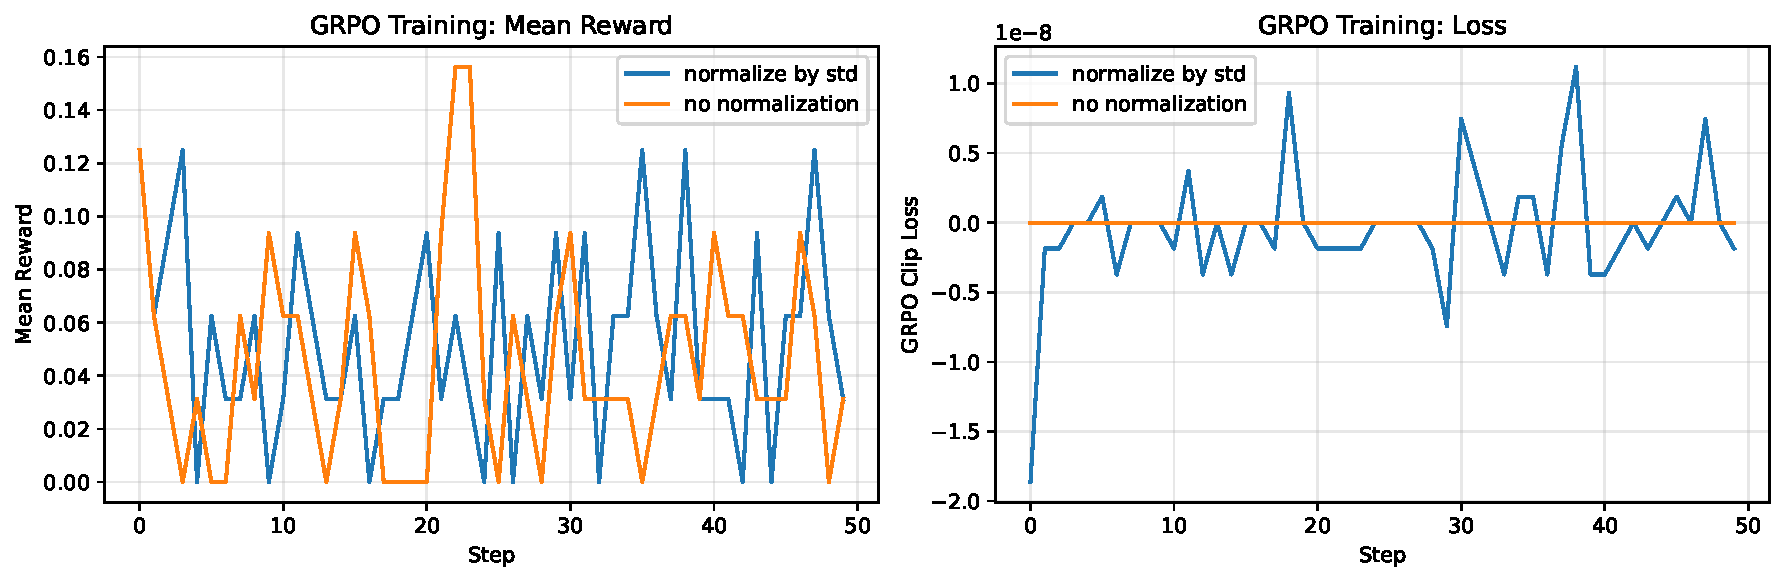
\includegraphics[width=0.9\textwidth]{grpo_curves.pdf}
\caption{GRPO training: mean reward (left) and GRPO clip loss (right) over 50 steps for both normalization variants.}
\label{fig:grpo}
\end{figure}

\end{document}
